\documentclass{beamer}
\usepackage{minted}
\usepackage{tikz}
\usetikzlibrary{shadows} 
\usetikzlibrary{positioning}
\usepackage{graphicx}
\usepackage{amssymb}
\usepackage{fontawesome}
\usepackage{xcolor}
\usepackage{pifont}
\usepackage{multirow}

\usepackage{colortbl}
\usetheme{Boadilla}

\newcommand{\greencheck}{{\color{green}\checkmark}}
\newcommand{\xmark}{\color{red}\ding{55}}

\title{Clojure for Data Scientists}
\subtitle{Unleash your data analysis passion }
\author{Cristiano Migliorini}
\institute{Vescore Academy}
\date{\today}

\begin{document}
\begin{frame}
\titlepage
\end{frame}

\begin{frame}
\frametitle{Foreword: Imperative vs Declarative Programming}

\begin{block}{Problem}
	Oder Name =[c,b,a] by Value=[3,2,1]
\end{block}


	\begin{columns}
		\begin{column}{0.5\textwidth}
	Imperative 
	\begin{itemize}
		\item indexing
		\item low abstraction
		\item procedural
	\end{itemize}
	Ideal for ordered numerical structures \\ 
	\begin{itemize}
		\item Order Value to NewValue=[1,2,3]
		\item Find the logical indexing to [3,2,1]
		\item Apply logical index to Name  [a,b,c]
	\end{itemize}
		\end{column}
		\begin{column}{0.5\textwidth}
	Declarative
	\begin{itemize}
		\item data collections
		\item high abstraction
		\item purely functional
	\end{itemize}
	Ideal for data and web applications
	\begin{itemize}
		\item Create collection [(v 3 n c)(v 2 n b)(v 1 n a)]
		\item Sort by v [(v 1 n a)(v 2 n b)(v 3 n c)]
		\item Extract n [a b c] \\

	\end{itemize}
		\end{column}
		\end{columns}
	\begin{block}{Declarative requirements: immutability and native hash-maps}
	\end{block}

\end{frame}


\begin{frame}[fragile]
\frametitle{Implementation of Foreword}

\begin{columns}
	\begin{column}{0.6\textwidth}
		\begin{center}
			\begin{minted}[fontsize=\scriptsize,escapeinside=||,mathescape=true]{clojure}
(def values '(3 2 1))

(def names '(c b a))

(def value-name (zipmap names values))

(keys (sort-by val < value-name))


; keywords are defined with : 
; Keywords are often used as keys in maps 
; and they provide faster comparisons 
; and lower memory overhead than strings

			\end{minted}
		\end{center}
	\end{column}
	\begin{column}{0.3\textwidth}
		\begin{minted}[fontsize=\scriptsize,escapeinside=||,mathescape=true]{text}
; values=> (3 2 1)
; java integer

; names=> (c b a) 
; java string

; value-name {c 3, b 2, a 1}
; sorted {a 1, b 2, c 3}
; extract keys (a b c)


; native hashmaps!
; value-name is 
; an abstraction!
		\end{minted}
	\end{column}
\end{columns}

	\begin{block}{Clojure edge}
You can do this with any good language (e.g. scala,kotlin) ...\\
...Clojure makes it easy (hash native) and efficient (immutability)...\\
...and it is implemented as LISP!
\end{block}


\end{frame}


\begin{frame}
\frametitle{Motivation}

\begin{itemize}

	\item Clojure is hosted on Java.
	\begin{itemize}
		\item 6 million developers, 15 billion devices
		\item Java provides unparalleled reliability, speed and performance
	\end{itemize}
	
	\item []
	\item ClojureScript is hosted on Browsers and Node.js
	\begin{itemize}
		\item building fast and scalable web and network applications
	\end{itemize}
\item []
	\item For developers and data Scientists
\begin{itemize}
	\item higher abstraction thinking, useful in any language
	\item inherently multi-threading, high performance
	\item highly reasuable code, high readability, higher productivity
	\item higher compensation (expert users switch to Clojure)
	\item used by innovative tech and fintech companies
\end{itemize}


\end{itemize}


\end{frame}


\begin{frame}
\frametitle{Outline}
\tableofcontents
\end{frame}

\section{Conceptual Foundation}

\subsection{Immutability}

\begin{frame}[fragile]
\frametitle{Immutability is a core design feature}

\begin{block}{Take away}
	Clojure is build on a powerful set of immutable, persistent, collection types.
	Core data structures are immutable.
\end{block}

\begin{itemize}
	\item Core data structures are immutable.
	\begin{itemize}
		\item Clojure is build on a powerful set of immutable, persistent, collection types.
	\end{itemize}
	
	
	\item Immutability is made easy. In Java it requires gymnastics.
	\begin{itemize}
		\item Working with immutable structures without complexity of their implementation. 
	\end{itemize}
\end{itemize}


\end{frame}

\begin{frame}[fragile]
\frametitle{Benefits of Immutability}


\textcolor{blue}{Pros}
\begin{itemize}
\item Data analysis logic is exposed

\begin{itemize}
	\item Trail of data transformation
\end{itemize}


\item Equality has meaning

\begin{itemize}
	\item Concurrent multi-threaded operations are meaningful
\end{itemize}

\item Sharing is efficient

\begin{itemize}
	\item Optimized Red-Black tree algorithms avoid copying
\end{itemize}

\end{itemize}

\textcolor{red}{Cons}
\begin{itemize}
\item Cost of Abstraction
\end{itemize}	



\end{frame}


\begin{frame}[fragile]

\frametitle{Equality and Identity are different}



\begin{columns}
\begin{column}{0.6\textwidth}
\begin{center}
	\begin{minted}[fontsize=\scriptsize,escapeinside=||,mathescape=true]{clojure}
(def fruit (list :apple :pear))
(def exotic-mix (cons :ananas fruit))
(def horror-mix (cons :potato fruit))
(def fruit-test (list :apple :pear))
	
(= (next exotic-mix)  (next horror-mix))
(= (next exotic-mix)  fruit-test)
	
(identical? (next exotic-mix)  (next horror-mix))
(identical? (next exotic-mix)  fruit-test)
\end{minted}
\end{center}
\end{column}
\begin{column}{0.3\textwidth}
\begin{minted}[fontsize=\scriptsize,escapeinside=||,mathescape=true]{text}
Fruit list is created
adds Anasas on Fruit
adds Potato on Fruit

next removes first element
true - equal
true -identical to Fruit

true - equal
|\color{red} false|


\end{minted}
\end{column}
\end{columns}
\end{frame}


\subsection{Namespace}
\begin{frame}
\frametitle{The Namespace}


\begin{columns}
\begin{column}{0.6\textwidth}
\begin{center}

\tikzset{every picture/.style={line width=0.75pt}} %set default line width to 0.75pt        

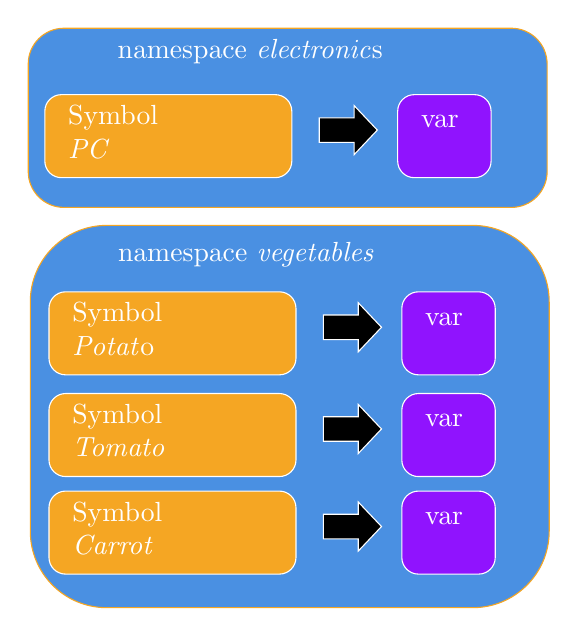
\begin{tikzpicture}[x=0.75pt,y=0.75pt,yscale=-1,xscale=1]
%uncomment if require: \path (0,312); %set diagram left start at 0, and has height of 312

%Rounded Rect [id:dp7797217429096077] 
\draw  [color={rgb, 255:red, 245; green, 166; blue, 35 }  ,draw opacity=1 ][fill={rgb, 255:red, 74; green, 144; blue, 226 }  ,fill opacity=1 ] (1,36.27) .. controls (1,26.73) and (8.73,19) .. (18.27,19) -- (233.73,19) .. controls (243.27,19) and (251,26.73) .. (251,36.27) -- (251,88.07) .. controls (251,97.6) and (243.27,105.33) .. (233.73,105.33) -- (18.27,105.33) .. controls (8.73,105.33) and (1,97.6) .. (1,88.07) -- cycle ;
%Rounded Rect [id:dp4101299877169058] 
\draw  [color={rgb, 255:red, 255; green, 255; blue, 255 }  ,draw opacity=1 ][fill={rgb, 255:red, 245; green, 166; blue, 35 }  ,fill opacity=1 ] (9,59) .. controls (9,54.58) and (12.58,51) .. (17,51) -- (120,51) .. controls (124.42,51) and (128,54.58) .. (128,59) -- (128,83) .. controls (128,87.42) and (124.42,91) .. (120,91) -- (17,91) .. controls (12.58,91) and (9,87.42) .. (9,83) -- cycle ;
%Rounded Rect [id:dp9819828475835948] 
\draw  [color={rgb, 255:red, 255; green, 255; blue, 255 }  ,draw opacity=1 ][fill={rgb, 255:red, 144; green, 19; blue, 254 }  ,fill opacity=1 ] (179,59) .. controls (179,54.58) and (182.58,51) .. (187,51) -- (216,51) .. controls (220.42,51) and (224,54.58) .. (224,59) -- (224,83) .. controls (224,87.42) and (220.42,91) .. (216,91) -- (187,91) .. controls (182.58,91) and (179,87.42) .. (179,83) -- cycle ;
%Right Arrow [id:dp6838296337081795] 
\draw  [color={rgb, 255:red, 255; green, 255; blue, 255 }  ,draw opacity=1 ][fill={rgb, 255:red, 0; green, 0; blue, 0 }  ,fill opacity=1 ] (141.2,62.17) -- (158,62.17) -- (158,56.25) -- (169.2,68.08) -- (158,79.92) -- (158,74) -- (141.2,74) -- cycle ;
%Rounded Rect [id:dp6138068621317438] 
\draw  [color={rgb, 255:red, 245; green, 166; blue, 35 }  ,draw opacity=1 ][fill={rgb, 255:red, 74; green, 144; blue, 226 }  ,fill opacity=1 ] (2,150.83) .. controls (2,130.49) and (18.49,114) .. (38.83,114) -- (215.17,114) .. controls (235.51,114) and (252,130.49) .. (252,150.83) -- (252,261.33) .. controls (252,281.68) and (235.51,298.17) .. (215.17,298.17) -- (38.83,298.17) .. controls (18.49,298.17) and (2,281.68) .. (2,261.33) -- cycle ;
%Rounded Rect [id:dp48323302418064285] 
\draw  [color={rgb, 255:red, 255; green, 255; blue, 255 }  ,draw opacity=1 ][fill={rgb, 255:red, 245; green, 166; blue, 35 }  ,fill opacity=1 ] (11,154) .. controls (11,149.58) and (14.58,146) .. (19,146) -- (122,146) .. controls (126.42,146) and (130,149.58) .. (130,154) -- (130,178) .. controls (130,182.42) and (126.42,186) .. (122,186) -- (19,186) .. controls (14.58,186) and (11,182.42) .. (11,178) -- cycle ;
%Rounded Rect [id:dp31869157730202335] 
\draw  [color={rgb, 255:red, 255; green, 255; blue, 255 }  ,draw opacity=1 ][fill={rgb, 255:red, 144; green, 19; blue, 254 }  ,fill opacity=1 ] (181,154) .. controls (181,149.58) and (184.58,146) .. (189,146) -- (218,146) .. controls (222.42,146) and (226,149.58) .. (226,154) -- (226,178) .. controls (226,182.42) and (222.42,186) .. (218,186) -- (189,186) .. controls (184.58,186) and (181,182.42) .. (181,178) -- cycle ;
%Right Arrow [id:dp7517089742742045] 
\draw  [color={rgb, 255:red, 255; green, 255; blue, 255 }  ,draw opacity=1 ][fill={rgb, 255:red, 0; green, 0; blue, 0 }  ,fill opacity=1 ] (143.2,157.17) -- (160,157.17) -- (160,151.25) -- (171.2,163.08) -- (160,174.92) -- (160,169) -- (143.2,169) -- cycle ;
%Rounded Rect [id:dp6196193689378513] 
\draw  [color={rgb, 255:red, 255; green, 255; blue, 255 }  ,draw opacity=1 ][fill={rgb, 255:red, 245; green, 166; blue, 35 }  ,fill opacity=1 ] (11,203) .. controls (11,198.58) and (14.58,195) .. (19,195) -- (122,195) .. controls (126.42,195) and (130,198.58) .. (130,203) -- (130,227) .. controls (130,231.42) and (126.42,235) .. (122,235) -- (19,235) .. controls (14.58,235) and (11,231.42) .. (11,227) -- cycle ;
%Rounded Rect [id:dp30364737175359013] 
\draw  [color={rgb, 255:red, 255; green, 255; blue, 255 }  ,draw opacity=1 ][fill={rgb, 255:red, 144; green, 19; blue, 254 }  ,fill opacity=1 ] (181,203) .. controls (181,198.58) and (184.58,195) .. (189,195) -- (218,195) .. controls (222.42,195) and (226,198.58) .. (226,203) -- (226,227) .. controls (226,231.42) and (222.42,235) .. (218,235) -- (189,235) .. controls (184.58,235) and (181,231.42) .. (181,227) -- cycle ;
%Right Arrow [id:dp6770715110186318] 
\draw  [color={rgb, 255:red, 255; green, 255; blue, 255 }  ,draw opacity=1 ][fill={rgb, 255:red, 0; green, 0; blue, 0 }  ,fill opacity=1 ] (143.2,206.17) -- (160,206.17) -- (160,200.25) -- (171.2,212.08) -- (160,223.92) -- (160,218) -- (143.2,218) -- cycle ;
%Rounded Rect [id:dp3164178476364725] 
\draw  [color={rgb, 255:red, 255; green, 255; blue, 255 }  ,draw opacity=1 ][fill={rgb, 255:red, 245; green, 166; blue, 35 }  ,fill opacity=1 ] (11,250) .. controls (11,245.58) and (14.58,242) .. (19,242) -- (122,242) .. controls (126.42,242) and (130,245.58) .. (130,250) -- (130,274) .. controls (130,278.42) and (126.42,282) .. (122,282) -- (19,282) .. controls (14.58,282) and (11,278.42) .. (11,274) -- cycle ;
%Rounded Rect [id:dp5911737271541524] 
\draw  [color={rgb, 255:red, 255; green, 255; blue, 255 }  ,draw opacity=1 ][fill={rgb, 255:red, 144; green, 19; blue, 254 }  ,fill opacity=1 ] (181,250) .. controls (181,245.58) and (184.58,242) .. (189,242) -- (218,242) .. controls (222.42,242) and (226,245.58) .. (226,250) -- (226,274) .. controls (226,278.42) and (222.42,282) .. (218,282) -- (189,282) .. controls (184.58,282) and (181,278.42) .. (181,274) -- cycle ;
%Right Arrow [id:dp15025518840518992] 
\draw  [color={rgb, 255:red, 255; green, 255; blue, 255 }  ,draw opacity=1 ][fill={rgb, 255:red, 0; green, 0; blue, 0 }  ,fill opacity=1 ] (143.2,253.17) -- (160,253.17) -- (160,247.25) -- (171.2,259.08) -- (160,270.92) -- (160,265) -- (143.2,265) -- cycle ;

% Text Node
\draw (42.83,23) node [anchor=north west][inner sep=0.75pt]   [align=left] {\textcolor[rgb]{1,1,1}{namespace \textit{electronic}s}};
% Text Node
\draw (19,55) node [anchor=north west][inner sep=0.75pt]   [align=left] {\textcolor[rgb]{1,1,1}{Symbol}\\\textit{\textcolor[rgb]{1,1,1}{PC}}};
% Text Node
\draw (189,60) node [anchor=north west][inner sep=0.75pt]  [color={rgb, 255:red, 255; green, 255; blue, 255 }  ,opacity=1 ] [align=left] {var};
% Text Node
\draw (21,150) node [anchor=north west][inner sep=0.75pt]   [align=left] {\textcolor[rgb]{1,1,1}{Symbol}\\\textcolor[rgb]{1,1,1}{\textit{Potat}o}};
% Text Node
\draw (191,155) node [anchor=north west][inner sep=0.75pt]  [color={rgb, 255:red, 255; green, 255; blue, 255 }  ,opacity=1 ] [align=left] {var};
% Text Node
\draw (21,199) node [anchor=north west][inner sep=0.75pt]   [align=left] {\textcolor[rgb]{1,1,1}{Symbol}\\\textcolor[rgb]{1,1,1}{\textit{Tomato}}};
% Text Node
\draw (191,204) node [anchor=north west][inner sep=0.75pt]  [color={rgb, 255:red, 255; green, 255; blue, 255 }  ,opacity=1 ] [align=left] {var};
% Text Node
\draw (21,246) node [anchor=north west][inner sep=0.75pt]   [align=left] {\textcolor[rgb]{1,1,1}{Symbol}\\\textcolor[rgb]{1,1,1}{\textit{Carrot}}};
% Text Node
\draw (191,251) node [anchor=north west][inner sep=0.75pt]  [color={rgb, 255:red, 255; green, 255; blue, 255 }  ,opacity=1 ] [align=left] {var};
% Text Node
\draw (43,121) node [anchor=north west][inner sep=0.75pt]   [align=left] {\textcolor[rgb]{1,1,1}{namespace \textit{vegetables}}};


\end{tikzpicture}

\end{center}
\end{column}
\begin{column}{0.3\textwidth}
\begin{itemize}
\item Namespace maps symbols to variables.

\item Namespace largely replaces the object in OOP. 
\end{itemize}
\end{column}
\end{columns}



\begin{tikzpicture}

\end{tikzpicture}



\end{frame}




\subsection{Homoiconicity}
\begin{frame}[fragile]
\frametitle{Clojure code is homoiconic: textual representation of lists}


\begin{columns}
	\begin{column}{0.6\textwidth}
		\begin{center}

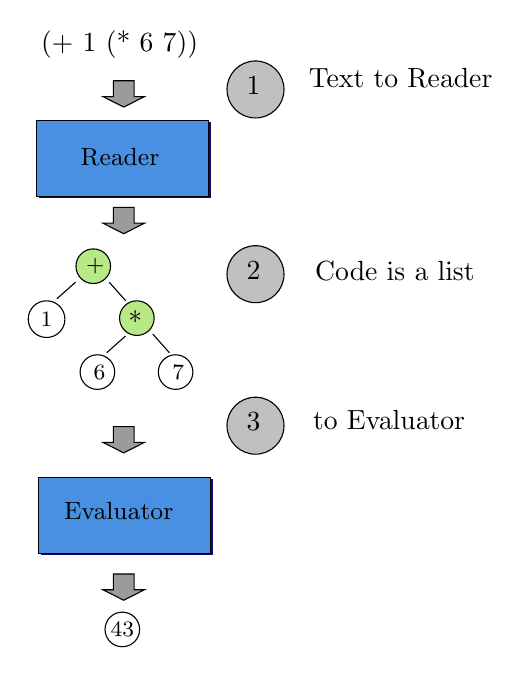
\begin{tikzpicture}[x=0.75pt,y=0.75pt,yscale=-1,xscale=1]
%uncomment if require: \path (0,322); %set diagram left start at 0, and has height of 322

%Shape: Circle [id:dp5426531940861452] 
\draw   (8,151.17) .. controls (8,146.29) and (11.95,142.33) .. (16.83,142.33) .. controls (21.71,142.33) and (25.67,146.29) .. (25.67,151.17) .. controls (25.67,156.05) and (21.71,160) .. (16.83,160) .. controls (11.95,160) and (8,156.05) .. (8,151.17) -- cycle ;
%Shape: Circle [id:dp47110567502885226] 
\draw  [fill={rgb, 255:red, 184; green, 233; blue, 134 }  ,fill opacity=1 ] (31,125.67) .. controls (31,121.06) and (34.73,117.33) .. (39.33,117.33) .. controls (43.94,117.33) and (47.67,121.06) .. (47.67,125.67) .. controls (47.67,130.27) and (43.94,134) .. (39.33,134) .. controls (34.73,134) and (31,130.27) .. (31,125.67) -- cycle ;
%Shape: Circle [id:dp9029398825984187] 
\draw  [fill={rgb, 255:red, 184; green, 233; blue, 134 }  ,fill opacity=1 ] (52,150.67) .. controls (52,146.06) and (55.73,142.33) .. (60.33,142.33) .. controls (64.94,142.33) and (68.67,146.06) .. (68.67,150.67) .. controls (68.67,155.27) and (64.94,159) .. (60.33,159) .. controls (55.73,159) and (52,155.27) .. (52,150.67) -- cycle ;
%Shape: Rectangle [id:dp42072904381429876] 
\draw  [fill={rgb, 255:red, 74; green, 144; blue, 226 }  ,fill opacity=1 ][general shadow={fill={rgb, 255:red, 18; green, 6; blue, 114 }  ,shadow xshift=0.75pt,shadow yshift=-0.75pt, opacity=1 }] (12,55.33) -- (95,55.33) -- (95,92) -- (12,92) -- cycle ;
%Down Arrow [id:dp8210637353714194] 
\draw  [fill={rgb, 255:red, 155; green, 155; blue, 155 }  ,fill opacity=1 ] (44,104.93) -- (49,104.93) -- (49,97.33) -- (59,97.33) -- (59,104.93) -- (64,104.93) -- (54,110) -- cycle ;
%Shape: Circle [id:dp3238596167029595] 
\draw   (33,176.67) .. controls (33,172.06) and (36.73,168.33) .. (41.33,168.33) .. controls (45.94,168.33) and (49.67,172.06) .. (49.67,176.67) .. controls (49.67,181.27) and (45.94,185) .. (41.33,185) .. controls (36.73,185) and (33,181.27) .. (33,176.67) -- cycle ;
%Shape: Circle [id:dp8892561535133561] 
\draw   (70.67,176.67) .. controls (70.67,172.06) and (74.4,168.33) .. (79,168.33) .. controls (83.6,168.33) and (87.33,172.06) .. (87.33,176.67) .. controls (87.33,181.27) and (83.6,185) .. (79,185) .. controls (74.4,185) and (70.67,181.27) .. (70.67,176.67) -- cycle ;
%Straight Lines [id:da9660485898011923] 
\draw    (47,133.33) -- (55,142.33) ;
%Shape: Boxed Line [id:dp8104208747623127] 
\draw    (21.83,141.33) -- (30.83,133.33) ;
%Shape: Boxed Line [id:dp9137192756939854] 
\draw    (45.83,167.33) -- (54.83,159.33) ;
%Straight Lines [id:da009103580572576098] 
\draw    (68,158.33) -- (76,167.33) ;
%Down Arrow [id:dp950812659228258] 
\draw  [fill={rgb, 255:red, 155; green, 155; blue, 155 }  ,fill opacity=1 ] (44,43.93) -- (49,43.93) -- (49,36.33) -- (59,36.33) -- (59,43.93) -- (64,43.93) -- (54,49) -- cycle ;
%Down Arrow [id:dp6092605854368234] 
\draw  [fill={rgb, 255:red, 155; green, 155; blue, 155 }  ,fill opacity=1 ] (44,210.53) -- (49,210.53) -- (49,202.93) -- (59,202.93) -- (59,210.53) -- (64,210.53) -- (54,215.6) -- cycle ;
%Shape: Rectangle [id:dp16142765621694544] 
\draw  [fill={rgb, 255:red, 74; green, 144; blue, 226 }  ,fill opacity=1 ][general shadow={fill={rgb, 255:red, 18; green, 6; blue, 114 }  ,shadow xshift=0.75pt,shadow yshift=-0.75pt, opacity=1 }] (13,227.33) -- (96,227.33) -- (96,264) -- (13,264) -- cycle ;
%Down Arrow [id:dp6856571303622645] 
\draw  [fill={rgb, 255:red, 155; green, 155; blue, 155 }  ,fill opacity=1 ] (44,281.53) -- (49,281.53) -- (49,273.93) -- (59,273.93) -- (59,281.53) -- (64,281.53) -- (54,286.6) -- cycle ;
%Shape: Circle [id:dp33799230215014453] 
\draw   (45,300.67) .. controls (45,296.06) and (48.73,292.33) .. (53.33,292.33) .. controls (57.94,292.33) and (61.67,296.06) .. (61.67,300.67) .. controls (61.67,305.27) and (57.94,309) .. (53.33,309) .. controls (48.73,309) and (45,305.27) .. (45,300.67) -- cycle ;

% Text Node
\draw (32,67.33) node [anchor=north west][inner sep=0.75pt]  [font=\small] [align=left] {Reader};
% Text Node
\draw (40.33,125.67) node  [font=\footnotesize,rotate=-0.98,xslant=-0.02] [align=left] {+};
% Text Node
\draw (16.83,151.17) node  [font=\footnotesize,rotate=-0.98,xslant=-0.02] [align=left] {1};
% Text Node
\draw (42.33,176.67) node  [font=\footnotesize,rotate=-0.98,xslant=-0.02] [align=left] {6};
% Text Node
\draw (80.33,176.9) node  [font=\footnotesize,rotate=-0.98,xslant=-0.02] [align=left] {7};
% Text Node
\draw (13,11) node [anchor=north west][inner sep=0.75pt]   [align=left] {(+ 1 (* 6 7))};
% Text Node
\draw  [fill={rgb, 255:red, 155; green, 155; blue, 155 }  ,fill opacity=0.63 ]  (117.5, 40.5) circle [x radius= 13.73, y radius= 13.73]   ;
\draw (112,33) node [anchor=north west][inner sep=0.75pt]   [align=left] {1};
% Text Node
\draw (142,29) node [anchor=north west][inner sep=0.75pt]   [align=left] {Text to Reader};
% Text Node
\draw  [fill={rgb, 255:red, 155; green, 155; blue, 155 }  ,fill opacity=0.63 ]  (117.5, 129.5) circle [x radius= 13.73, y radius= 13.73]   ;
\draw (112,122) node [anchor=north west][inner sep=0.75pt]   [align=left] {2};
% Text Node
\draw (145,122) node [anchor=north west][inner sep=0.75pt]   [align=left] {Code is a list};
% Text Node
\draw  [fill={rgb, 255:red, 155; green, 155; blue, 155 }  ,fill opacity=0.63 ]  (117.5, 202.5) circle [x radius= 13.73, y radius= 13.73]   ;
\draw (112,195) node [anchor=north west][inner sep=0.75pt]   [align=left] {3};
% Text Node
\draw (144,194) node [anchor=north west][inner sep=0.75pt]   [align=left] {to Evaluator};
% Text Node
\draw (53.33,300.67) node  [font=\footnotesize,rotate=-0.98,xslant=-0.02] [align=left] {43};
% Text Node
\draw (24,238.33) node [anchor=north west][inner sep=0.75pt]  [font=\small] [align=left] {Evaluator};
% Text Node
\draw (55,146) node [anchor=north west][inner sep=0.75pt]    {$*$};


\end{tikzpicture}
		\end{center}
\end{column}
\begin{column}{0.5\textwidth}
			\begin{minted}[fontsize=\scriptsize,escapeinside=||,mathescape=true]{clojure}

; invoke the reader
(read-string "(+ 1 2)")
; (+ 1 2) as list


; invoke the reader
(read-string "#(+ 1 %)")
; (fn* [p1__27183#] (+ 1 p1__27183#)) 




; eval evaluates the list
; using the Java Virtual Machine
(eval '(+ 1 2))
;3
\end{minted}
\end{column}
\end{columns}


\end{frame}


\begin{frame}[fragile]
\frametitle{Clojure Special forms}

\begin{block}{Take away}
The first position in a list is the "calling" position (typicall a function).
It can also be:
	\begin{itemize}
		\item a special form: def, defn (fn), if, quote, throw, try, loop, recur, let,...
		\item a macro
		\end{itemize}
\end{block}


\begin{columns}
	\begin{column}{0.5\textwidth}
		\begin{center}
			\begin{minted}[fontsize=\scriptsize,escapeinside=||,mathescape=true]{clojure}
(def
 ^{:doc "bla bla "
 :user/comment "extra comment"}
 my-var 1)

(def 
 ^{:private false
 :doc "my help"
 :user/comment "this is the best fn ever!"
 :namespace "main"} 
 my-private-var 1)

(meta #'my-private-var)
;(meta (var my-private-var))
			\end{minted}
		\end{center}
	\end{column}
	\begin{column}{0.5\textwidth}
		\begin{minted}[fontsize=\scriptsize,escapeinside=||,mathescape=true]{clojure}
;def special form to define variable
;def ^{metadata} variable value

;special attention to:
; :private, makes the variable private!
; :namespace, again, scoping
		
		\end{minted}
	\end{column}
\end{columns}

\end{frame}

\begin{frame}[fragile]
\frametitle{Clojure Special forms}


\begin{columns}
	\begin{column}{0.5\textwidth}
		\begin{center}
			\begin{minted}[fontsize=\scriptsize,escapeinside=||,mathescape=true]{clojure}
(defn sum2 [x1 x2]
 (+ x1 x2))

(defn sum3
 ([x1 x2] (+ x1 x2))
 ([x1 x2 x3] (+ (+ x1 x2) x3)))
 
(defn example
 {:doc "test"
 :test #(do 
 (assert (= (example 1) 2))
 (assert (= (example -1) -2)))}
 [i] i)
 
(test #'example)

(defn constrained-sqr [x]
 {:pre  [(pos? x)]
 :post [(> % 16), (< % 225)]}
(* x x))



			\end{minted}
		\end{center}
	\end{column}
	\begin{column}{0.5\textwidth}
		\begin{minted}[fontsize=\scriptsize,escapeinside=||,mathescape=true]{clojure}
;define function, 2 inputs
;(sum2  1 3) => 4

;multi-arity, 2 or 3 inputs
;(sum3 1 2 ) => 3
;(sum3 1 2 3)=> 6

;asssertion tests are quite frequent




;throws error


; pre-post work like interceptors
(constrained-sqr 4)  => error
(constrained-sqr -1) => error
(constrained-sqr 10) => 100 ;ok
		
		\end{minted}
	\end{column}
\end{columns}

\end{frame}


\begin{frame}[fragile]
\frametitle{Clojure syntax is extended by macros}
\begin{columns}
	\begin{column}{0.5\textwidth}
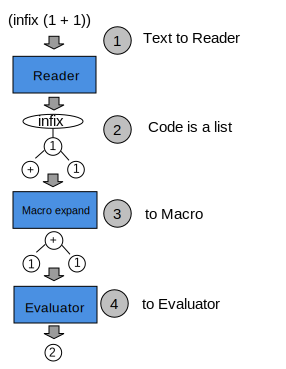
\includegraphics[scale=0.6]{macro.png}
	\end{column}
\begin{column}{0.5\textwidth}
	\begin{minted}[fontsize=\scriptsize,escapeinside=||,mathescape=true]{clojure}
;the macro takes lists and symbols
;unlike a function does not evaluate	
(defmacro infix
 [infixed]
 (list (second infixed)
 (first infixed)
 (last infixed)))

(infix (1 + 1))
;2
 
; just to understand !
(macroexpand '(infix (1 + 1)))
; the macro returns the list
;(+ 1 1) 
	
	
(eval '(+ 1 1))
;2
	
	\end{minted}
	
\end{column}
\end{columns}
\end{frame}

\begin{frame}[fragile]
\frametitle{Macros syntax}
\begin{columns}
	\begin{column}{0.5\textwidth}
		\begin{minted}[fontsize=\tiny,escapeinside=||,mathescape=true]{clojure}
; first write your goal
(if (> 5 1)  (do (print "yes") (print "!") 10))

; then traslate it into a macro
(defmacro my-when [condition & body]
 (list 'if condition
 (concat (list 'do) body)))

; check that macro is correctly written
(macroexpand '(my-when (> 5 1)  (print "yes") (print "!") 10))
;(if (> 5 1) (do (print "yes") (print "!") 10))

; it works
(my-when (> 5 1)  (print "yes") (print "!") 10) ; yes! 10

; same more compact
(defmacro my-when [pred & body]
`(if ~pred (do ~@body) ))

(my-when-2 (> 5 1) (print "yes") (print "!") 10) ; yes! 10

; `syntax quoting fully qualified symbols, enables unquote ~
; ~  unquote (aka substitute)
; ~@ unquote splicing (aka removes parenthesis)

`(1 2 (+ 3 4))      ;(1 2 (clojure.core/+ 3 4))
`(1 2 ~(+ 3 4))     ;(1 2 7)

`(+ ~(list 1 2 3))  ;(clojure.core/+ (1 2 3))
`(+ ~@(list 1 2 3)) ;(clojure.core/+ 1 2 3) , removes ()

		
		\end{minted}
	\end{column}
	\begin{column}{0.5\textwidth}
	\begin{minted}[fontsize=\scriptsize,escapeinside=||,mathescape=true]{clojure}
		\end{minted}
\end{column}
\end{columns}
\end{frame}


\begin{frame}
\frametitle{Collections in Clojure}
\begin{columns}
\begin{column}{0.5\textwidth}
\begin{center}
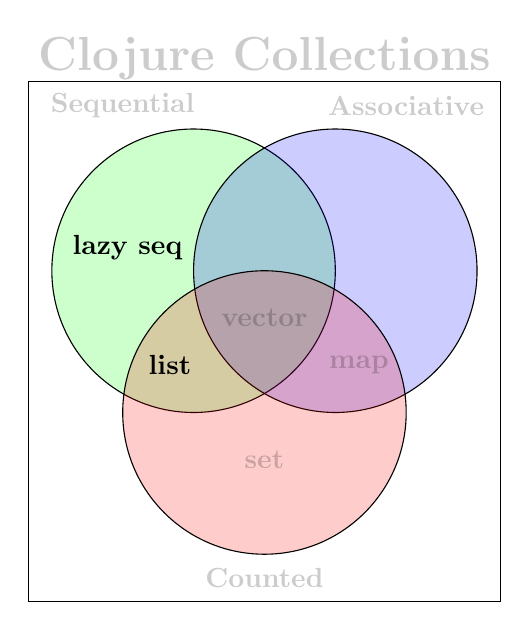
\begin{tikzpicture}[scale=0.6]
%% You can adjust the opacity here. For venn diagrams it is convenient to have a low opacity so that you can see intersections
\begin{scope} [fill opacity = .2]
%% The draw command knows a lot of shapes. To make a rectangle you just need to specify two diagonal corners. Make sure you always have a semicolon at the end of your draw commands, otherwise latex flips out.
\draw (-5,5) rectangle (5,-6);
%% Similarly, you can make a circle by specifying the center and then the radius. You can also add a fill color, but if you're printing in black and white you'll probably want to remove that line.
\draw[fill=green, draw = black] (-1.5,1) circle (3);
\draw[fill=blue, draw = black] (1.5,1) circle (3);
\draw[fill=red, draw = black] (0,-2) circle (3);
%% We can use the node command to label points. If you put your cursor on "LARGE" or "textbf" a box will drop down with size and text style options.
\node at (0,5.5) {\LARGE\textbf{Clojure Collections}};
\node at (-3,4.5)  {\textbf{Sequential}};
\node at (3,4.5)   {\textbf{Associative}};
\node at (0,-5.5) {\textbf{Counted}};
\node at (0,-3) {\textbf{set}};
\node at (0,-0) {\textbf{vector}};
\node at (2,-1) {\textbf{map}};
\end{scope}
\node at (-2,-1) {{\textbf{list}}};
\node at (-2.9,1.5) {\textbf{lazy seq}};
%% And now you have a venn diagram. Yay!
%\draw[help lines](-5,5) grid (5,-6);    This line can draw the grid lines to help guide you. I use these when I'm writing the code and then delete this line when I publish the pdf.
\end{tikzpicture}
\end{center}
\end{column}

\begin{column}{0.5\textwidth}
	\begin{center}
		
\begin{itemize}
\item Vectors are both sequential \emph{and} associative
\item Sets are neither sequential \emph{nor} associative
\item Discover object type:
\begin{itemize}
	\item coll?  IPersistentCollection 
	\item counted?  finite or infinite 
	\item associative?  key-value
	\item sequential? linearly ordered
\end{itemize}
	\item can be read in sequences
	\item list and lazy seq are already sequences
\end{itemize}
	\end{center}
\end{column}	
\end{columns}
\end{frame}

\subsection{Sequence Abstraction}

\begin{frame}[fragile]
\frametitle{Treating Lists*, Vectors, Sets, and Maps as Sequences}

\begin{block}{Take away}
	sequence is a collection of elements organized in linear order
\end{block}

Sequable objects, can be cast in a sequence
\begin{itemize}
	\item Clojure Collections
	\begin{itemize}
		\item Maps (aka hashes or dictionaries)
		\item Vectors
		\item Sets
		\item Lists
		\begin{itemize}
			\item singly linked lists
			\item by default are sequences
			\item head access
			\item Clojure code is represented by lists
		\end{itemize}
		
	\end{itemize}
	
	\item Java Maps,array, strings
	\item Java Iterable
	\item Java Collections
	\item Java Sequable
\end{itemize}

\end{frame}

\begin{frame}[fragile]
\frametitle{Sequence Abstraction}

Operation definitions work on \textit{different} collection types

\begin{itemize}
	\item a sequable data structure is similar to linked list 
	\item a sequence can be walked through with  first, rest and cos
	\item linear-access functions derive a seq from their argument  
	\begin{itemize}
	\item[]	$\Rightarrow$ \textbf{functions work on any data type}
	\end{itemize}
	\item sequence are parsed one element at the time, are often lazy
\end{itemize}

\begin{minted}[fontsize=\scriptsize,escapeinside=||,mathescape=true]{text}


(map #(* 2 %) [1 2 3])
(map #(* 2 %) '(1 2 3))
(map #(* 2 %)  (sorted-set 1 2 3))
; the data structure is different, vector, list, map

(seq [1 2 3])
(seq '(1 2 3))
(seq (sorted-set 1 2 3))
; the underlying sequence is the same (1 2 3)
; this is why map works on vector, list, map returns (2 4 6)
(seq {:a 1 :b 1})
;even a map will be sequable ([:a 1] [:b 1])

\end{minted}
\end{frame}


\begin{frame}[fragile]
\frametitle{Putting it all together}
\begin{table}
	\begin{center}
		\scalebox{0.6}{
\begin{tabular}{|l|c|c|c|c|c|c|c|c|} 
	\cline{2-9}
	\multicolumn{1}{l|}{} & \multicolumn{6}{c|}{ \cellcolor{blue!25} \textbf{Collections}}  & \multicolumn{2}{c|}{\cellcolor{blue!15} \textbf{Other Objects}} \\ 
	\cline{2-9}
	\multicolumn{1}{l|}{} & \cellcolor{green!15} List & \cellcolor{green!5}Vector & \cellcolor{blue!5}Map & \cellcolor{pink!25}Set &\cellcolor{gray!5} Seq (stringSeq)& \cellcolor{gray!5} Lazy Seq (iterate) & \cellcolor{gray!5}String  & \cellcolor{gray!5}nil  \\  \hline
\cellcolor{blue!25} \textbf{Operations }      & '(1 2 3)    & [4 5 6]     & \{:a 1, :b 2\} & \#\{7 8 9\} & (seq "hello")  & (range)     & "hello"      & nil    \\ \hline
	seq?                  & \greencheck & \xmark      & \xmark         & \xmark      & \greencheck    & \greencheck & \xmark       &\xmark  \\ \hline
	coll?                 & \greencheck & \greencheck & \greencheck    & \greencheck & \greencheck    & \greencheck & \xmark       & \xmark \\ \hline
	counted?              & \greencheck & \greencheck & \greencheck    & \greencheck & \greencheck    & \xmark (infinite) & \xmark & \xmark \\ \hline
	sequential?           & \greencheck & \greencheck & \xmark         & \xmark      & \greencheck    & \greencheck       & \xmark  & \xmark \\ \hline
	associative?          & \xmark      & \greencheck & \greencheck    & \xmark      & \xmark         & \xmark            & \xmark & \xmark \\ \hline
\end{tabular}}
\end{center}
\end{table}

\begin{itemize}
\item derive a sequence backed by any collection using seq
\item vectors and ordered sets can be sequenced in reverse using rseq
\item read any sequence into a new collection
\item lists and vector are extremely interchangeable 
\end{itemize}

\end{frame}

\begin{frame}[fragile]
\frametitle{Putting it all together}
\begin{table}
		\begin{center}
	\scalebox{0.46}{
	%\begin{tabular}{lllllllll}
	\begin{tabular}{llccccccc}
		&                     &                &                    & \multicolumn{2}{c}{ \cellcolor{blue!15} Associative}                                                                         &                         &                      &             \\
		&                     &                & \multicolumn{2}{c}{\cellcolor{green!25} Sequential}        & (implicit)                                                                           &                         &                      &             \\ 
		\cline{2-9}
		& Description         &  Syntax         & List               & Vector           & Map                                                                                  & Set                     & Example              & Result      \\ 
		\hline
		\multirow{3}{*}{Create~} & Create coll         &                & (list 1 2)         & (vec 1 2)        & \begin{tabular}[c]{@{}l@{}}(hash-map :a 1 :b 2)\\(zipmap [:a :b] [1 2])\end{tabular} & (set '(1 2))            &                      &             \\
		& Create with Literal &                & '(1 2)             & {[}1 2]          & \{:a 1 :b 2\}                                                                        & \#\{1 2\}               &                      &             \\
		& Convert coll        &                & (apply list [1 2]) & (vec '(1 2))     &                                                      \xmark                                & (set '(1 2))            &                      &             \\ 
		\hline
		\multirow{3}{*}{Merge}   & Conversion  Merge   & (into to from) & (into () [1 2])    & (into [] '(1 2)) &    \xmark                                                        & (into \#\{\} [1 2 3]) &                      &             \\
		& Merge (allow mixed) & (concat x y)   &     \greencheck               &   \greencheck               &                               \greencheck                                                       &        \greencheck                 & (concat [1 2] [3 4]) & (1 2 3 4)   \\
		& Merge  &  (merge \& maps)   &    \greencheck   &    \greencheck    &  \greencheck  & \greencheck  & 
		 (merge [1 2] 3 4) & [1 2 3 4]  \\
		\hline
	\end{tabular}}
		\end{center}
\end{table}

\end{frame}

\begin{frame}[fragile]
\frametitle{Putting it all together}
\begin{table}
	\begin{center}
			\scalebox{0.5}{
	\begin{tabular}{llccccccc}
		&   &   &     &   \multicolumn{2}{l}{ \cellcolor{blue!15} Associative} &   &  &   \\
		&       &     & \multicolumn{2}{l}{\cellcolor{green!25} Sequential}   & (implicit) &      &  &  \\ 
		\cline{2-9}
		& Description     & Syntax                   & List        & Vector                     & Map        & Set                & Example                         & Result         \\
		\cline{1-9}
		\multirow{4}{*}{Add}    & Add Elements    & (con coll x  xs)         & first       & last                       &      \greencheck      &      \greencheck              & (conj [1 2] [3 4])              & {[}1 2 [3 4]]  \\
		& Add Multiple    & (assoc map key val  kvs) &  \xmark  &      \greencheck      &   \greencheck  &   \xmark    & (assoc [1 2] 2 '[3 5])          & {[}1 2 [3 4]]  \\
		& Append*         & (append coll x  xs)      &   \greencheck  &  \greencheck &    \xmark         &       \xmark              & (append '(1 2) 3 4)             & {[}1 2 3 4]    \\
		& Preprend*       & (prepend x  xs coll)     &  \greencheck &  \greencheck   &       \xmark      &         \xmark            & (prepend 3 4 [1 2])             & {[}3 4 1 2]    \\ 
		\hline
		\multirow{3}{*}{Remove} & Remove Multiple & (remove pred coll)       &  \greencheck   &     \greencheck   &   \greencheck \xmark     &        \greencheck \xmark              & (remove pos? [1 -2])            & (-2)           \\
		& Remove          & (dissoc map key)         &    \xmark   &  \xmark   &   \greencheck  &  \xmark          & (dissoc \{:a 1 :b 2 :c 3\} :b\} & \{:a 1 :c 3\}  \\
		& Remove Start   & (drop n coll)            &   \greencheck          &       \greencheck                     &    \greencheck        &         \xmark            & (drop 1 \{:a 1 :b 2\})          & ([:b 2])       \\ 
		\hline
		\multirow{2}{*}{Stack}  & Peek            &                          &  Get first           &         Get Last                   &    \xmark         &              \xmark       &                                 &                \\
		& Pop             &                          & Drop first & Drop last &        \xmark     &   \xmark        &                                 &                \\
		\cline{1-9}
	\end{tabular}	}
		
		
	\end{center}
\end{table}
* Tupelo
\end{frame}




\begin{frame}[fragile]
\frametitle{Putting it all together}


\begin{table}
		\begin{center}
		\scalebox{0.42}{
			
\begin{tabular}{llccccccc}
	&      &     &      &    \multicolumn{2}{c}{ \cellcolor{blue!15} Associative} & &                                                                                                                                                                                                                                                                                                                                                                                           &  \\
				&             &                                                                                      & \multicolumn{2}{c}{\cellcolor{green!25}Sequential}                                                                               & (implicit) &                    &                                                                                                                                                                                                                                                                                                                                                                                                                                                                        &                                                                                                                                                                                          \\ 
				\cline{2-9}
				& Description & Syntax                                                                               & List & Vector                                                                                                & Map        & Set                & Example                                                                                                                                                                                                                                                                                                                                                                                                                                                                & Result                                                                                                                                                                                   \\ 
				\hline
				\multirow{2}{*}{Access}    & Access ele  &                                                                                      & nth  & nth                                                                                                   & nth        & nth                & (nth \#\{1 2 3\} 1)                                                                                                                                                                                                                                                                                                                                                                                                                                                    & 2 - throws error                                                                                                                                                                         \\
				& Access ele  &                                                                                      & get  & get                                                                                                   & get        & get                & (get \{:a 1 :b 2\} :b)                                                                                                                                                                                                                                                                                                                                                                                                                                                 & 2 - throws nil                                                                                                                                                                           \\ 
				\hline
				\multirow{4}{*}{Subset}    & Subset      & (select-keys map keyseq)                                                             & \xmark     &  \greencheck                                                                                                      &   \greencheck          & \xmark                 & \begin{tabular}(select-keys \{:a 1 :b 2\}\\{[}:a :b]\}\end{tabular}                                                                                                                                                                                                                                                                                                                                                                                        & \{:a 1, :b 2\}                                                                                                                                                                           \\
				& Subvec      & (subvec v start end)                                                                 &   \greencheck    &  \greencheck                                                                                                      &   \greencheck          &   \greencheck                 & (subvec [1 2 3 4] [2 3])                                                                                                                                                                                                                                                                                                                                                                                                                                               & {[}2 3 4]                                                                                                                                                                                \\
				& Indexing    & \begin{tabular}[c]{@{}l@{}}(keep-indexed f coll)\\or\\(map indexed ...)\end{tabular} &  \greencheck     & \begin{tabular}(keep-indexed \#(if (pos? \%2) \%1)~\\{[}-9 0 29 -7 45 3 -8])\end{tabular} &  \greencheck           &  \greencheck                   & \begin{tabular}[c]{@{}l@{}}(keep-indexed \#(if (odd? \%1) \%2)\\{[}:a :b :c :d :e])\end{tabular}                                                                                                                                                                                                                                                                                                                                                                       & (:b :d)                                                                                                                                                                                  \\
				& Replace     & (replace map coll)                                                                   &   \greencheck   &  \greencheck                                                                                                      &   \greencheck          & \xmark                   & (replace [10 9 8 7 6] [0 2 4])                                                                                                                                                                                                                                                                                                                                                                                                                                         & {[}10 8 6]                                                                                                                                                                               \\ 
				\hline
				Modify                     & Update      & (update m k f x)                                                                     & \xmark     &  \greencheck                                                                                                      &   \greencheck          & \xmark                  & (update [1 2] 0 / 3)                                                                                                                                                                                                                                                                                                                                                                                                                                                   & {[}1/3 2]                                                                                                                                                                                \\ 
				\hline
				\multirow{4}{*}{Transform} & Map         & (map f coll)     &   \greencheck   &   \greencheck                                                                                                     & \xmark          & \xmark                  & (map + [1 2 3] [4 5 6])                                                                                                                                                                                                                                                                                                                                                                                                                                                & (5 6 7)                                                                                                                                                                                  \\
				& Map-kv      & (map-kv f coll)**                                                                    & \xmark     &   \greencheck                                                                                                     &   \greencheck          & \xmark                   & (map + \{:a 1 :b 2\} \{:a 4 :b 5\})                                                                                                                                                                                                                                                                                                                                                                                                                                    & \{:a 5 :b 7\}                                                                                                                                                                            \\
				& Reduce      & (reduce f val coll)                                                                  &   \greencheck    &   \greencheck                                                                                                     & \xmark          &   \greencheck                  & (reduce + 1 ~[1 2])                                                                                                                                                                                                                                                                                                                                                                                                                                                    & 4                                                                                                                                                                                        \\
				& Reduce-kv   & (reduce-kv f init coll)                                                              &\xmark     & \xmark                                                                                                      &   \greencheck          & \xmark                   & \begin{tabular}(def num (vec (range 10))) \\ (reduce-kv (fn [s k v] \\ (if even? k) + s v) s)) 0 num)\end{tabular} & 20                                                                                                                                                                                       \\ 
				\hline
				Sort                       & Sort        & (sort-by val f coll)                            & \xmark     &  \greencheck                                                                                                      &   \greencheck          & \xmark                  & (sort-by val < {:a 3 :b 2})                                                                                                                                                                                                                   & ([:b 2][:a 3])  \\
				\hline
			\end{tabular}
			
			
}
\end{center}
\end{table}
** Medley
\end{frame}


\section{Common operations}
\subsection{Updating Structures}
\begin{frame}[fragile]
\frametitle{Update Data Strucures}


\begin{block}{Take away}
	Data type is not relevant !
\end{block}



\begin{columns}
	\begin{column}{0.5\textwidth}
		\begin{center}
			\begin{minted}[fontsize=\scriptsize,escapeinside=||,mathescape=true]{clojure}
(def matrix
 [[1 2 3]
 [3 4 5]
 [6 7 8]])
 
(assoc-in matrix [1 2] 'hello)
;assoc in data   [row col] value
			\end{minted}
		\end{center}
	\end{column}
	\begin{column}{0.5\textwidth}
		\begin{minted}[fontsize=\scriptsize,escapeinside=||,mathescape=true]{text}
			
[[1 2 3] [3 4 5] [6 7 8]]



[[1 2 3] [3 4 hello] [6 7 8]]
; this is powerful!

		\end{minted}
	\end{column}
\end{columns}


\end{frame}

\begin{frame}[fragile]
\frametitle{Update Hierachical Data Strucures}


\begin{block}{Take away}
	Data indexing is flexible!
\end{block}



\begin{columns}
	\begin{column}{0.5\textwidth}
		\begin{center}
			\begin{minted}[fontsize=\scriptsize,escapeinside=||,mathescape=true]{clojure}
(def matrix
  [[1 2 3]
   [3 4 5]
   [6 7 8]])
			
(def hyper-matrix
	(vec (concat [[[1 1] [2 2] [3 3]]]
	(subvec matrix 1))))
			
(identical? (get matrix 2) (get hyper-matrix 2))
; true, data are shared
			
(assoc-in hyper-matrix [0 1 1] 'hello)
;[[[1 1] [2 hello] [3 3]] [3 4 5] [6 7 8]]
			
(assoc-in hyper-matrix [1 1] 'hello)
;[[[1 1] [2 2] [3 3]] [3 hello 5] [6 7 8]]
			\end{minted}
		\end{center}
	\end{column}
	\begin{column}{0.5\textwidth}
		\begin{minted}[fontsize=\scriptsize,escapeinside=||,mathescape=true]{text}
			
      ;from a classical matrix 3x3
      [[1 2 3] [3 4 5] [6 7 8]]
			
			
      ;to this monster, sharing data
      [[[1 1] [2 2] [3 3]] 
      [3 4 5] [6 7 8]]
      ;this is powerful!
      
      
      
      ;indexing
      [fist sec sec]
			
			
      [sec sec]		
		\end{minted}
	\end{column}
\end{columns}

\end{frame}


\begin{frame}[fragile]
\frametitle{Bad design}
\begin{columns}
	\begin{column}{0.5\textwidth}
		\begin{center}
			\begin{minted}[fontsize=\scriptsize,escapeinside=||,mathescape=true]{clojure}
(def matrix
[[1 2 3]
[3 4 5]
[6 7 8]])


(def hyper-matrix
 (vec (concat [[[1 1] [2 2] [3 3]] 
 (rest matrix)])))
;[[[1 1] [2 2] [3 3]] ([3 4 5] [6 7 8])]


(def hyper-matrix
 (vec (concat [[[1 1] [2 2] [3 3]]] 
 (vec (rest matrix))))
;[[[1 1] [2 2] [3 3]] [3 4 5] [6 7 8]]
		
			\end{minted}
		\end{center}
	\end{column}
	\begin{column}{0.5\textwidth}
		\begin{minted}[fontsize=\scriptsize,escapeinside=||,mathescape=true]{text}
		
		
;same as before		
		
		
		
		


;this is now a hybrid structure
;difficult to work with





;this is now easily workable 



		\end{minted}
	\end{column}
\end{columns}

\begin{block}{Take away}
	Prewalk /postwalk can help, normally symptom of bad design
\end{block}


\end{frame}




\subsection{List Comprehension}

\begin{frame}[fragile]
\frametitle{For}

List comprehension. Repeatedly executes body and collects results calculated iteratively.

\begin{block}{Take away}
	Makes it is easy to generate a list
\end{block}



\begin{columns}
	\begin{column}{0.5\textwidth}
		\begin{center}
			\begin{minted}[fontsize=\scriptsize,escapeinside=||,mathescape=true]{clojure}
(for [i [1 2 3]]
 (inc i))
;(2 3 4)

(for [i [1 2 3]
      j [3 2 1]]
 [i j])
;([1 3] [1 2] ...)
			
			\end{minted}
		\end{center}
	\end{column}
	\begin{column}{0.5\textwidth}
		\begin{minted}[fontsize=\scriptsize,escapeinside=||,mathescape=true]{text}
iteration
result is collected


multiple index iteration
result is collected
		
		\end{minted}
	\end{column}
\end{columns}

\begin{block}{Doseq}
Doseq Repeatedly executes body but returns nil 
\end{block}

\end{frame}

\subsection{Destructuring}
\begin{frame}[fragile]
\frametitle{Destructuring}

\begin{block}{Let}
Let defines a local scope. Let-like expressions destructure (doseq, for).
\end{block}

\begin{columns}
	\begin{column}{0.6\textwidth}
		\begin{center}
			\begin{minted}[fontsize=\scriptsize,escapeinside=||,mathescape=true]{clojure}
(def x 2)

(let [x 3]
(println x))

(println x)

(def my-coll [[1 2] [3 4] {:a 1 :b 1} [8 9 10]])

(let [       [[x1 x2] p2  {p3 :a}    & rest 
 :as all] my-coll]
 (println x1)
 (println p2)
 (println p3)
 (println rest)
 all)


			
			\end{minted}
		\end{center}
	\end{column}
	\begin{column}{0.5\textwidth}
		\begin{minted}[fontsize=\scriptsize,escapeinside=||,mathescape=true]{text}
;x=2

;x in let will shadow x
;x=3

;x=2		


;read top down the code

;first vec hierachical, second vec
;then map, then rest
;1
;[3 4]
;1
;([8 9 10]) rest collection
[[1 2] [3 4] {:a 1, :b 1} [8 9 10]]
		\end{minted}
	\end{column}
\end{columns}
\end{frame}

\begin{frame}[fragile]
\frametitle{Destructuring Maps}

\begin{block}{Let}
	Also known as associative destructuring.
\end{block}

\begin{columns}
	\begin{column}{0.6\textwidth}
		\begin{center}
			\begin{minted}[fontsize=\tiny,escapeinside=||,mathescape=true]{clojure}
(doseq [[dim value] 
        {:width 1 :lenght 2 :depth 3}] 
   (println (str (name dim) ":" value)))
			
(let 
 [{a :length} {:width 1 :length 2 :weight 3}]
 (println a))	

;avoid keyname repetition
 (let [{:keys [width] } 
 {:width 1 :length 2 :weight 3}]
 (println width))
 
(def multiplayer-state
 {:joe {:class "A"
 :tool "B"
 :score "C"}
 :joa {:class "D"
 :tool "F"
 :score "G"}})
 
 (let [ {{:keys [class tool]} :joe} 
 multiplayer-state]
 (println tool))
			
			\end{minted}
		\end{center}
	\end{column}
	\begin{column}{0.5\textwidth}
		\begin{minted}[fontsize=\tiny,escapeinside=||,mathescape=true]{text}
;key-value vector, prints
;width:1
;lenght:2
;depth:3

;2




;1











;B









		\end{minted}
	\end{column}
\end{columns}




\end{frame}

\subsection{Apply}
\begin{frame}[fragile]
\frametitle{Apply}

Apply unwraps a sequence and applies the function to them as individual arguments

\begin{columns}
	\begin{column}{0.55\textwidth}
		\begin{center}
			\begin{minted}[fontsize=\scriptsize,escapeinside=||,mathescape=true]{clojure}
(apply + [1 2 3 4 5])


(apply map vector [[:a :b] [:c :d]])


(map #(apply max %) [[1 2 3][4 5 6][7 8 9]])
			
			
			\end{minted}
		\end{center}
	\end{column}
	\begin{column}{0.45\textwidth}
		\begin{minted}[fontsize=\scriptsize,escapeinside=||,mathescape=true]{clojure}
; removes the external brakets
; (+ 1 2 3 4 5) 
; 15

;(map vector [:a :b] [:c :d])
;([:a :c] [:b :d])

; map loop [1 2 3] [4 5 6] [7 8 9]	
;(apply max [1 2 3]) ... (max 1 2 3)
;(apply max [4 5 6]) ... (max 4 5 6)
;...
;(3 6 9)
		
		\end{minted}
	\end{column}
\end{columns}

\begin{block}{Take away}
	Often use in combination with map
\end{block}

\end{frame}

\subsection{Thread-first Macro}
\begin{frame}[fragile]
\frametitle{Thread-first Macro}

Inserts x as the second item in the first form.If there are more forms, inserts the first form as the second item in second form.

\begin{block}{Take away}
Makes code more readable left to right. Macro expands syntax!
\end{block}



\begin{columns}
	\begin{column}{0.1\textwidth}
		\begin{center}
		\begin{minted}[escapeinside=||,mathescape=true]{text}
              (->  |$\underbrace{x}$|
		|$\underbrace{ \text{(*         3)}}$|
		|$\underbrace{ \text{(/         5)}}$|
		(dec   ))
		
		
		\end{minted}
		    \end{center}
	\end{column}
	\begin{column}{0.7\textwidth}
		\begin{minted}[escapeinside=||,mathescape=true]{text}
		 x is a var, for example 10
		 10 multiplied by 3 
		 30 divided by 5
		 6 decreased by 1
		 
		 
		\end{minted}
	\end{column}
\end{columns}

\end{frame}

\begin{frame}[fragile]
\frametitle{Thread-first Thread-last debugging}

Use function (spy) from Tupelo library to print intermediary values


\begin{columns}
	\begin{column}{0.5\textwidth}
		\begin{center}
			\begin{minted}[fontsize=\scriptsize,escapeinside=||,mathescape=true]{clojure}	
(:use [tupelo.core])

-> 1
(inc)
(spy :after-inc)     
(* 2))

:after-inc => 2
4			

(->> 1
(inc)
(spy :after-inc)      
(* 2))

:after-inc => 2
4	
			\end{minted}
		\end{center}
	\end{column}
	\begin{column}{0.5\textwidth}
		\begin{minted}[fontsize=\scriptsize,escapeinside=||,mathescape=true]{clojure}
		
		
; add a custom keyword message






; spy with  ->  and  ->>  forms
		\end{minted}
	\end{column}
\end{columns}



\end{frame}


\begin{frame}[fragile]
\frametitle{Literate Thread Macro}

Use  Tupelo library to mix first and last


\begin{columns}
	\begin{column}{0.5\textwidth}
		\begin{center}
			\begin{minted}[fontsize=\scriptsize,escapeinside=||,mathescape=true]{clojure}	
(:use [tupelo.core])
			
(it-> 1
 (inc it)                                  
 (+ it 3)                                 
 (/ 10 it)                                 
 (str "We need to order " it " items." ))
 
(it-> 3
(spy :initial it)
(let [x it]
(spy x :xis3)
(inc x))
(spy it :itis4)
(* it 2)
(spyx it))


			\end{minted}
		\end{center}
	\end{column}
	\begin{column}{0.5\textwidth}
		\begin{minted}[fontsize=\scriptsize,escapeinside=||,mathescape=true]{clojure}

; thread-first or thread-last
; thread-first
; thread-last





;:initial => 3
;:xis3 => 3
;:itis4 => 4
;it => 8
;8
		
		\end{minted}
	\end{column}
\end{columns}



\end{frame}

\subsection{State management}
\begin{frame}[fragile]
\frametitle{Atom: Syncronous Uncoordinated State Management}

\begin{block}{Take away}
	Atom guarantees thread-safe state management
\end{block}


\begin{columns}
	\begin{column}{0.5\textwidth}
		\begin{center}
			\begin{minted}[fontsize=\scriptsize,escapeinside=||,mathescape=true]{clojure}
(defn single-thread-inc [] 
(def x 0)
(defn inc-x [] (def x (inc x)))
(doseq [_ (range 100)] (inc-x)) x)
(single-thread-inc)

(defn parallel-inc [] 
(def x 0)
(defn inc-x []  (future (def x (inc x))))
(doseq [_ (range 100)] (inc-x)) x)
(parallel-inc)

(defn parallel-inc-v2 [] 
(def x (atom 0))
(defn inc-x []  (future (swap! x inc)))
(doseq [_ (range 100)] (inc-x)) x)
(parallel-inc-v2)
			\end{minted}
		\end{center}
	\end{column}
	\begin{column}{0.5\textwidth}
		\begin{minted}[fontsize=\scriptsize,escapeinside=||,mathescape=true]{clojure}
; single -thread execution
;x => 100


;future triggers multi-threads
; x => is random between 0 and 100
; every state works on a different x



; Atom manages the update of the variable
; x is always 100!
; Atom Syntax is simple
; (def atom-int (atom 53))
; (reset! atom-int 35)
; (swap! atom-int inc)

; deref or @ to get value
		
		
		\end{minted}
	\end{column}
\end{columns}



\end{frame}

\section{Documentation}
\subsection{Doc}

\begin{frame}[fragile]
\frametitle{Documentation}


\begin{block}{Take away}
	Keeping the comment close to code is easy!
\end{block}



\begin{columns}
	\begin{column}{0.5\textwidth}
		\begin{center}
			\begin{minted}[fontsize=\scriptsize,escapeinside=||,mathescape=true]{clojure}

(:use [clojure.repl])

(def my-variable "This is unity" 1)

(defn print-input "This prints the input" [s]
      (println s))

(doc my-variable)

(find-doc "unity")
			\end{minted}
		\end{center}
	\end{column}
	\begin{column}{0.3\textwidth}
		\begin{minted}[fontsize=\scriptsize,escapeinside=||,mathescape=true]{text}
Doc is from clojure.repl








-----------------
main/my-variable
This is unity

-----------------
main/my-variable
This is unity

		\end{minted}
	\end{column}
\end{columns}


\end{frame}


\section{Performance}
\subsection{Immutability and Abstraction costs}

\begin{frame}[fragile]
\frametitle{Abstraction}
Clojure abstraction and immutability requires overhead operations

\begin{columns}
	\begin{column}{0.5\textwidth}
		\begin{center}
			\begin{minted}[fontsize=\scriptsize,escapeinside=||,mathescape=true]{clojure}
(ns main
(:require [clojure.string :as str]
          [criterium.core :as cc]))


(let [s "ab"]
     (cc/quick-bench (= "ab" s))
     (cc/quick-bench (.equals "ab" s)))

(let [s (str "a" "b")]
     (cc/quick-bench (= "ab" s))
     (cc/quick-bench (.equals "ab" s)))
			\end{minted}
		\end{center}
	\end{column}
	\begin{column}{0.5\textwidth}
		\begin{minted}[fontsize=\scriptsize,escapeinside=||,mathescape=true]{text}

Execution time mean





 3.2 ns
 3.5 ns


|\color{red} 45.2 ns|
 7.4 ns

		\end{minted}
	\end{column}
\end{columns}
\end{frame}



\subsection{Recursion}

\begin{frame}[fragile]
\frametitle{Recursive expressions}
Let us take a tour on Factorial without and with recursion

\begin{columns}
	\begin{column}{0.5\textwidth}
		\begin{center}
			\begin{minted}[fontsize=\scriptsize,escapeinside=||,mathescape=true]{clojure}
(defn factorial [n]
(reduce * (range 1 (inc n))))
;reduce multiply on a vector

(defn factorial [n]
(second (last (take (inc n) 
(iterate 
    (fn [[a b]] [(inc a) (* a b)]) 
         [1 1])))))
;easy approach for formulas

(defn factorial [n]
(if (< n 2) 1
(* n (factorial (dec n)))))
;classic recursion


			\end{minted}
		\end{center}
	\end{column}
	\begin{column}{0.5\textwidth}
		\begin{minted}[fontsize=\scriptsize,escapeinside=||,mathescape=true]{text}
		
 Execution time mean
	
 190 ns

		
		
			
|\color{red} 1560 ns|





 250 ns
		
		\end{minted}
	\end{column}
\end{columns}
\end{frame}


\begin{frame}[fragile]
\frametitle{Tail Recursion}

In tail recursion the last call is a recursion to the function

\begin{block}{Take away}
	Tail recursion runs without new stack frames
\end{block}

\begin{itemize}
	\item A helper function, with an extra accumulator argument
	\item A break point to exit
	\item A recur (or loop-recur)
\end{itemize}	



\begin{columns}
	\begin{column}{0.6\textwidth}
		\begin{center}
			\begin{minted}[fontsize=\scriptsize,escapeinside=||,mathescape=true]{clojure}
(defn factorial
  ([n] (factorial n 1)) ;or [m]
  ([n acc]              ;and (loop [n m acc 1]
      (if  (< n 2) acc
      (recur (dec n) (* acc n)))))		
			\end{minted}
		\end{center}
	\end{column}
	\begin{column}{0.5\textwidth}
		\begin{minted}[fontsize=\scriptsize,escapeinside=||,mathescape=true]{text}
		
Execution time mean 215 ns
Arity-1 to call Arity-2, helper fun	
Arity-2
break point if n=1 return acc = n!
recur [n-1 1*n],[n-2 1*n*(n-1)],...		
		\end{minted}
	\end{column}
\end{columns}
\end{frame}


\section{Maps}
\subsection{Payload design considerations}

\begin{frame}[fragile]
\frametitle{Map Design}

\begin{block}{Take away}
	The structure of the map must be taylored to its function
\end{block}

\begin{columns}
	\begin{column}{0.6\textwidth}
		\begin{center}
Database and API Payloads\\		
\vspace{0.5cm}			
\underline{Vector of Flat Maps}		
			\begin{minted}[fontsize=\scriptsize,escapeinside=||,mathescape=true]{text}
			
[{:type a :cat :equity :pref ['LP' 'MS']},
{:type b :cat :fx :pref ['BB' 'LP']},...]	
			\end{minted}
		\end{center}
\begin{itemize}
	\item share common keys
	\item keep datalog/datom structure
\end{itemize}
	\end{column}
	\begin{column}{0.5\textwidth}
		\\
		\vspace{0.5cm}
		App State Management\\		
		\vspace{0.5cm}			
		\underline{Hierarchical Maps}	
		\begin{minted}[fontsize=\scriptsize,escapeinside=||,mathescape=true]{text}
{:waterfall 
  {:class 
   {:eq {:bd ['LP' 'MS']}
   {:fx {:bd ['BB' 'MS']}
   {:fi {:bd ['PM' 'MS']}}}}		
		\end{minted}
\begin{itemize}
	\item Re-frame
	\item Complexity Cost
\end{itemize}
	\end{column}
\end{columns}
\end{frame}


\begin{frame}[fragile]
\frametitle{Vector of Maps Inner Join}
\begin{columns}
	\begin{column}{0.6\textwidth}
		\begin{center}
			\begin{minted}[fontsize=\scriptsize,escapeinside=||,mathescape=true]{clojure}
(def map1 [{:id 1 :name "n1"}
{:id 2 :name "n2"}
{:id 3 :name "n3"}])

(def map2 [{:id 2 :address "a1"}
{:id 3 :address "a2"}
{:id 4 :address "a3"}])

(clojure.set/join map1 map2)
(print-table (clojure.set/join map1 map2))	
			\end{minted}
		\end{center}
	\end{column}
	\begin{column}{0.5\textwidth}
		\begin{minted}[fontsize=\scriptsize,escapeinside=||,mathescape=true]{text}
[|\color{red} {:id 1, :name "n1"} |
 {:id 2, :name "n2"} 
 {:id 3, :name "n3"}]
 
[{:id 2, :address "a1"} 
 {:id 3, :address "a2"} 
 |\color{red}{:id 4, :address "a3"}|]	
 
 | :id | :name | :address |
 |-----+-------+----------|
 |   2 |    n2 |       a1 |
 |   3 |    n3 |       a2 |
 
		\end{minted}
	\end{column}
\end{columns}

\end{frame}


\begin{frame}[fragile]
\frametitle{Vector of Maps Outer Join}
\begin{columns}
	\begin{column}{0.5\textwidth}
		\begin{center}
			\begin{minted}[fontsize=\tiny,escapeinside=||,mathescape=true]{clojure}
(clojure.set/union map1 map2)

;[{:id 1, :name "n1"}
;{:id 2, :name "n2"}
;{:id 3, :name "n3"}
;{:id 2, :address "a1"}
;{:id 3, :address "a2"}
;{:id 4, :address "a3"}]

(vals (clojure.set/index 
 (clojure.set/union map1 map2) [:id]))

;list of sets of maps...
;(#{{:id 1, :name "n1"}}
;#{{:id 2, :address "a1"} {:id 2, :name "n2"}}
;#{{:id 3, :name "n3"} {:id 3, :address "a2"}}
;#{{:id 4, :address "a3"}})

			\end{minted}
		\end{center}
	\end{column}
	\begin{column}{0.5\textwidth}
		\begin{minted}[fontsize=\tiny,escapeinside=||,mathescape=true]{clojure}
(concat map1 map2)

;({:id 1, :name "n1"}
;{:id 2, :name "n2"}
;{:id 3, :name "n3"}
;{:id 2, :address "a1"}
;{:id 3, :address "a2"}
;{:id 4, :address "a3"})

(vals (group-by :id 
 (concat map1 map2)))

;list of vectors of maps
;([{:id 1, :name "n1"}]
;[{:id 2, :name "n2"} {:id 2, :address "a1"}]
;[{:id 3, :name "n3"} {:id 3, :address "a2"}]
;[{:id 4, :address "a3"}])
		\end{minted}
	\end{column}
\end{columns}

\begin{center}
\begin{minted}[fontsize=\tiny,escapeinside=||,mathescape=true]{clojure}
(print-table [:id :name :address] (map #(apply merge %) ...) 
; or
(print-table [:id :name :address] (map #(reduce merge %) ...) 
\end{minted}
\begin{minted}[fontsize=\tiny,escapeinside=||,mathescape=true]{text}
| :id | :name | :address |
|-----+-------+----------|
|   1 |    n1 |          |
|   2 |    n2 |       a1 |
|   3 |    n3 |       a2 |
|   4 |       |       a3 |
\end{minted}	
\end{center}

\end{frame}


\begin{frame}[fragile]
\frametitle{Vector of Maps Outer Join}
\begin{columns}
	\begin{column}{0.5\textwidth}
		\begin{center}
			\begin{minted}[fontsize=\tiny,escapeinside=||,mathescape=true]{clojure}
(def new-map1 (zipmap (map :id map1) map1))





(def new-map2 (zipmap (map :id map2) map2))




(vals (merge-with merge new-map1 new-map2))



(print-table [:id :name :address] 
 (vals (merge-with merge new-map1 new-map2)))

			\end{minted}
		\end{center}
	\end{column}
	\begin{column}{0.5\textwidth}
		\begin{minted}[fontsize=\scriptsize,escapeinside=||,mathescape=true]{text}
;new map 1
; key - value: value is a map!
;{1 {:id 1, :name "n1"}, 
; 2 {:id 2, :name "n2"}, 
; 3 {:id 3, :name "n3"}}

;new map 2
; key - value: value is a map!
;{2  {:id 2, :address "a1"}, 
; 3  {:id 3, :address "a2"}, 
; 4  {:id 4, :address "a3"}}		

;list of maps
;({:id 1, :name "n1"} 
; {:id 2, :name "n2", :address "a1"} 
; {:id 3, :name "n3", :address "a2"} 
; {:id 4, :address "a3"})
 
; | :id | :name | :address |
; |-----+-------+----------|
; |   1 |    n1 |          |
; |   2 |    n2 |       a1 |
; |   3 |    n3 |       a2 |
; |   4 |       |       a3 |
		\end{minted}
	\end{column}
\end{columns}
\end{frame}

\end{document}


